% \s{有限温度における非磁性不純物効果}\label{sec:form:tmat}

\begin{figure}[t]
\begin{center}
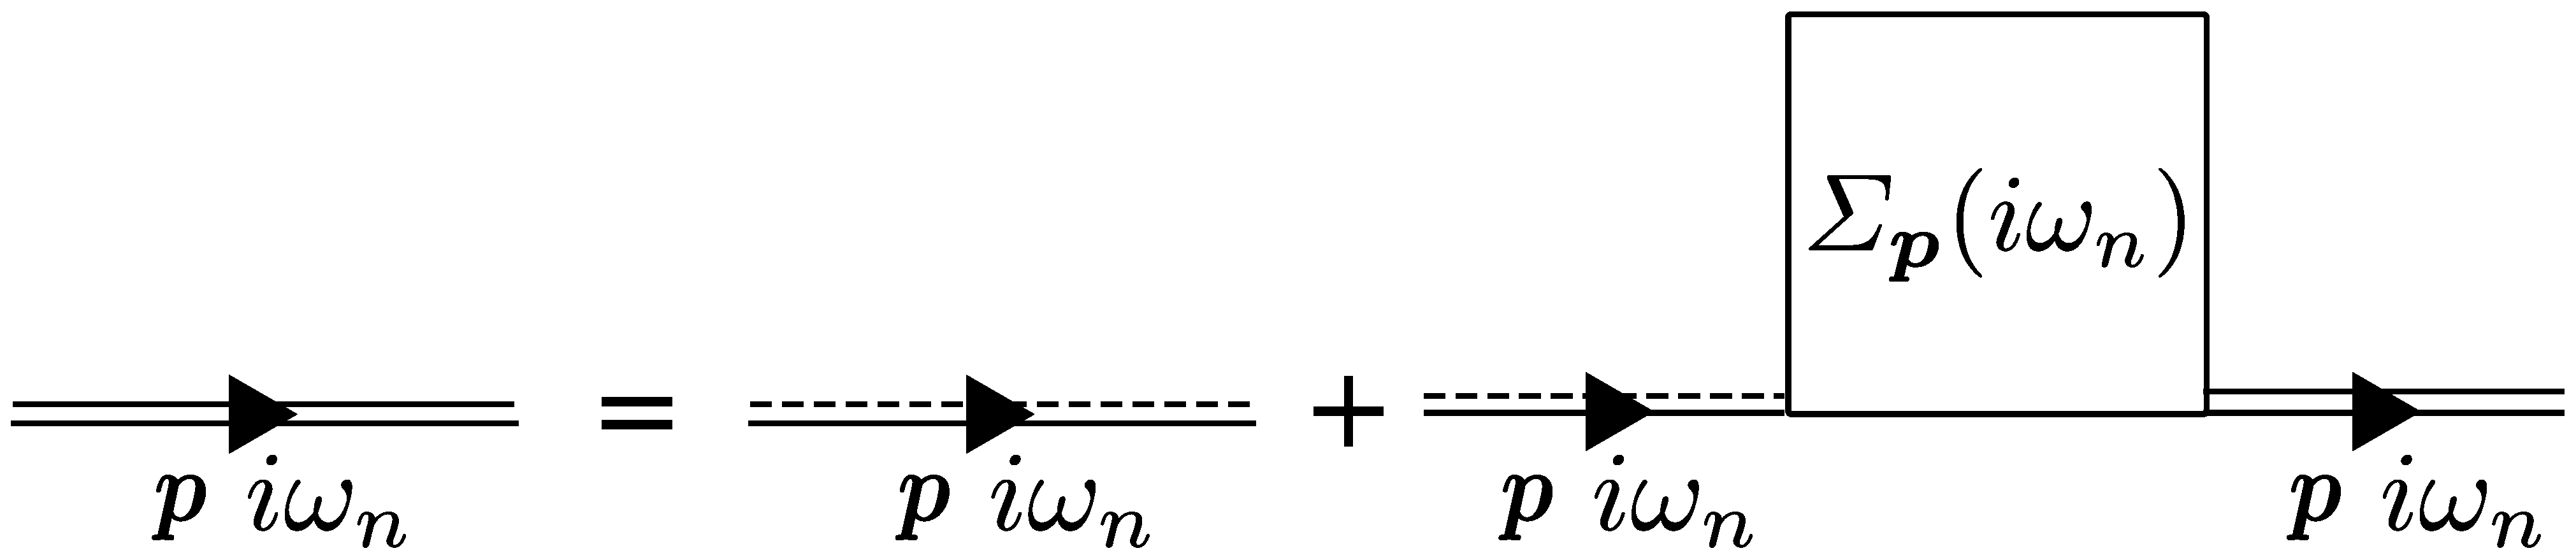
\includegraphics[height=20mm]{eps/dyson-tma-imp.eps}
\end{center}
\caption{原子間相互作用の効果を含む 1 粒子温度グリーン関数 $\gpom$ のダイソン方程式。二重実線は $\gpom$、破線と実線による二重線は不純物グリーン関数 $\gimppom$、$\sigpom$ は引力相互作用の効果を表す自己エネルギーである。}
\label{fig:form:tma:greenall}
\end{figure}


\begin{figure}[t]
\centering
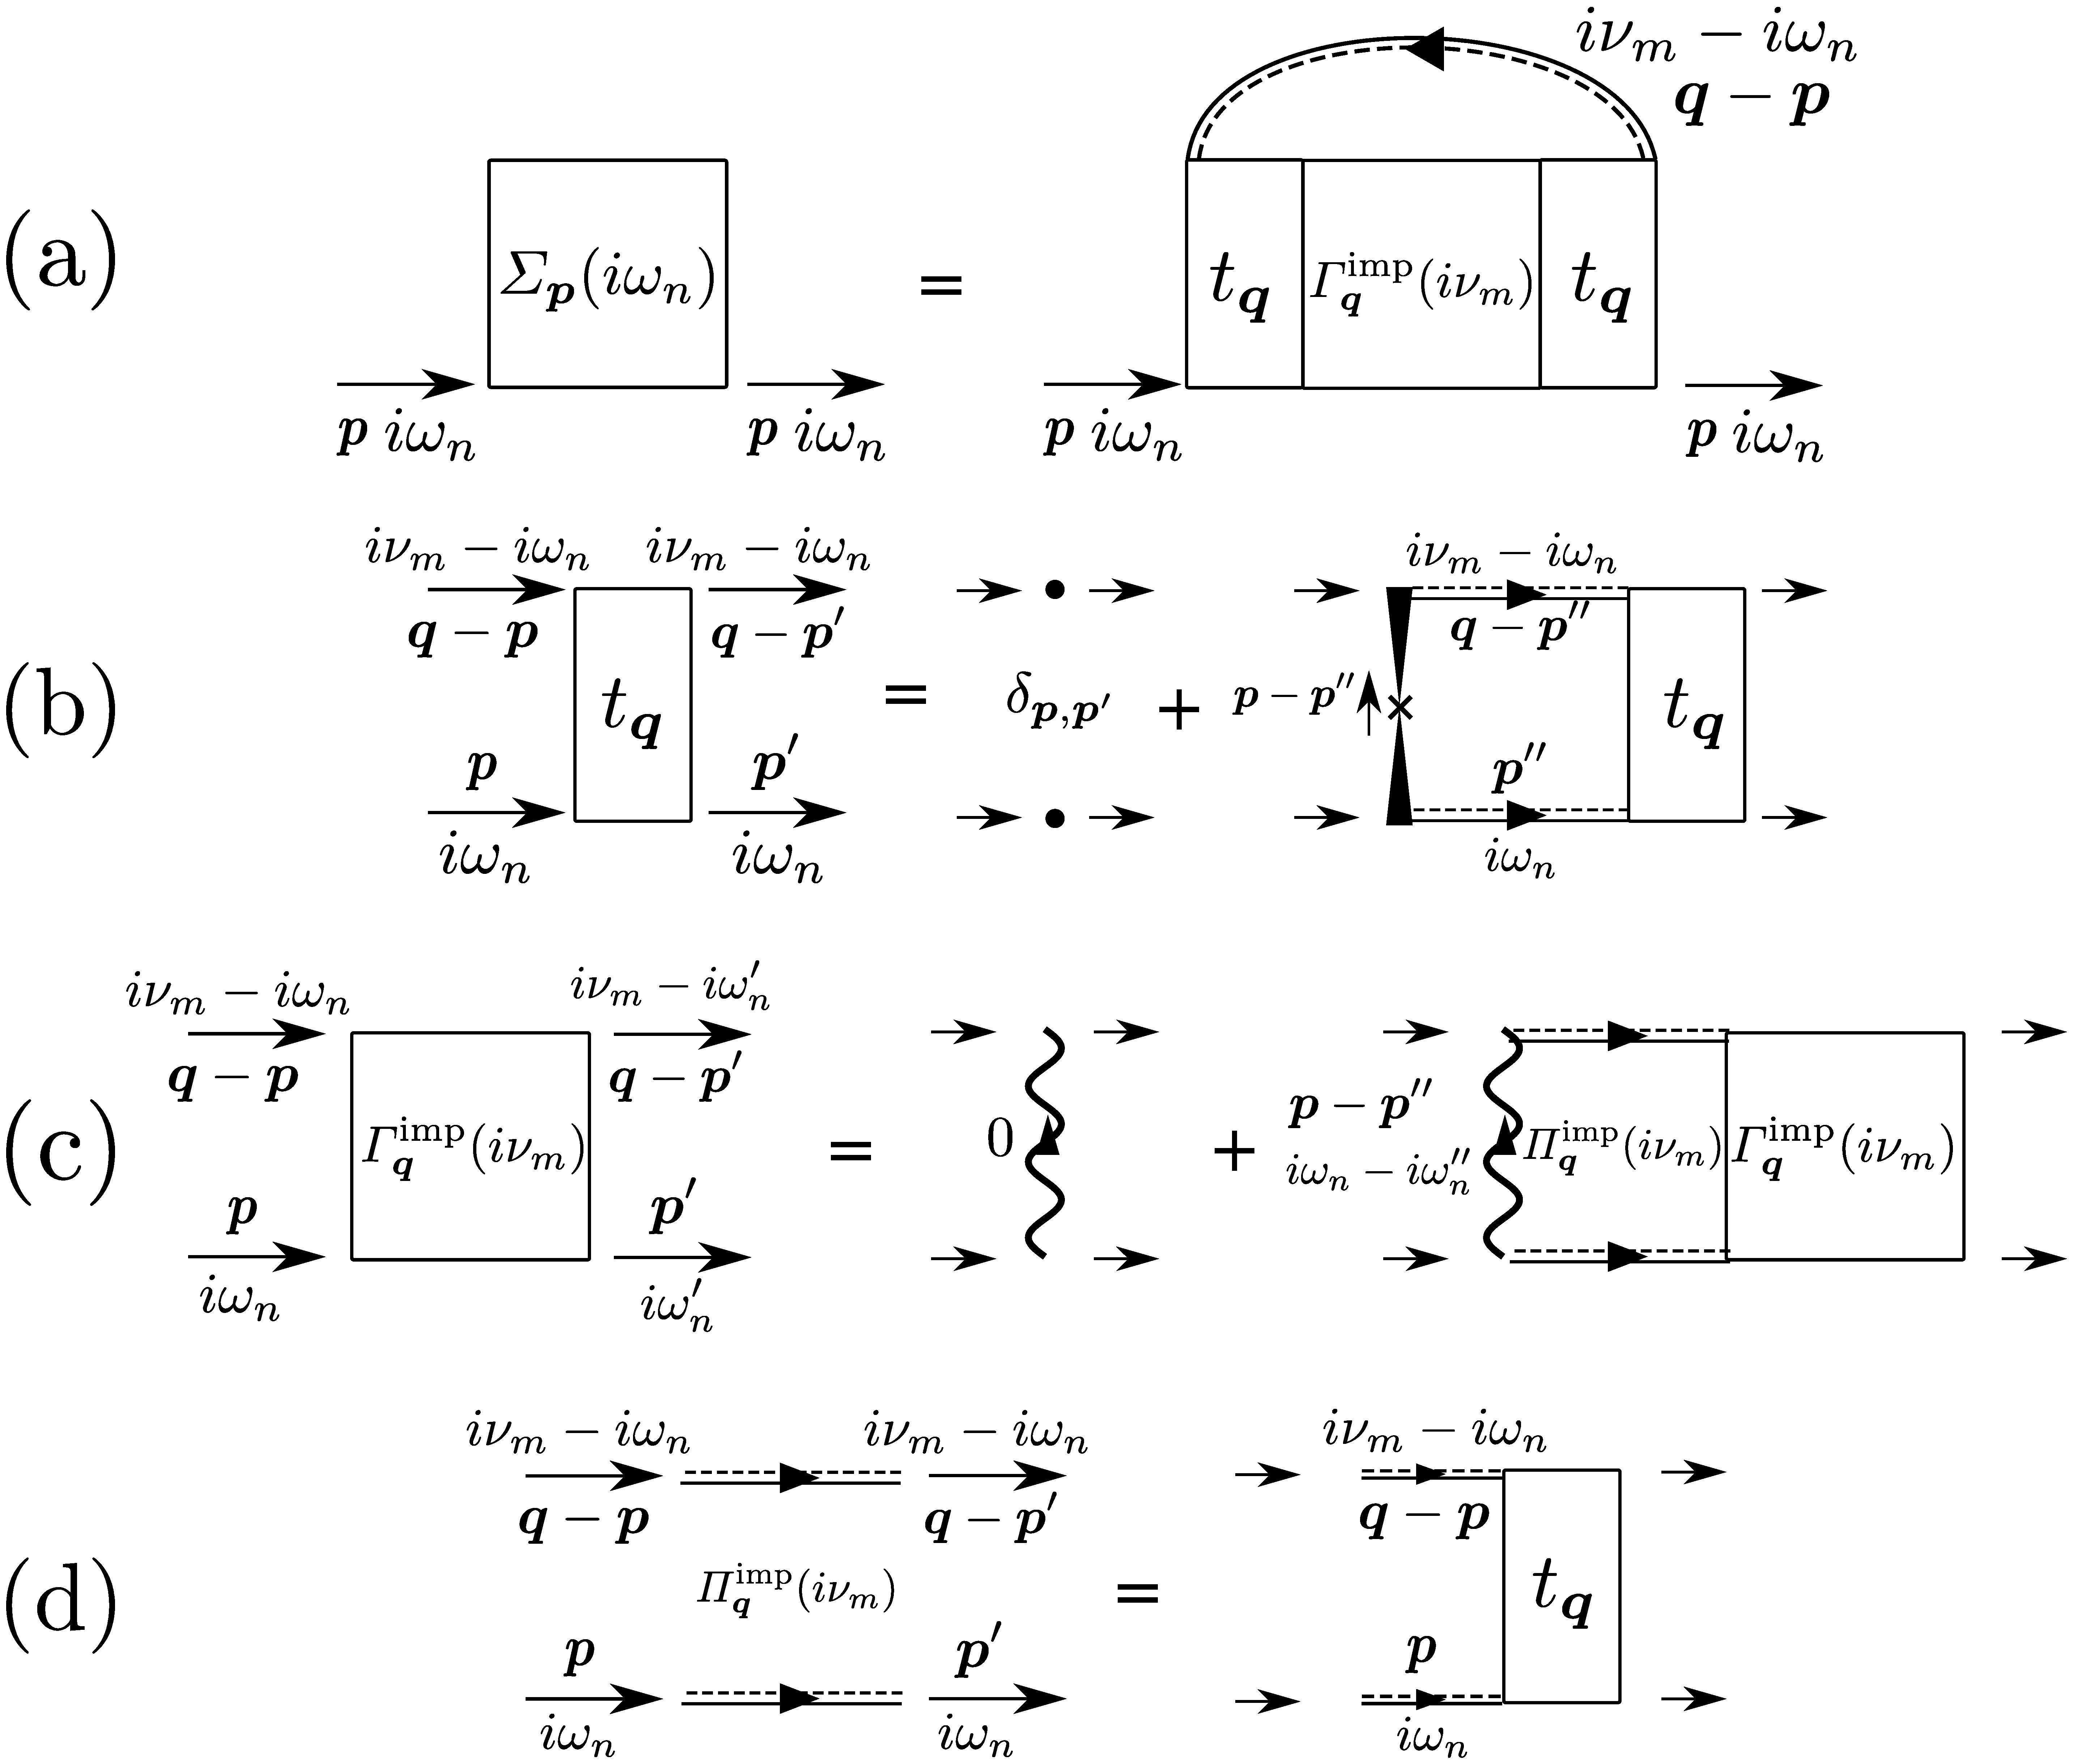
\includegraphics[width=123mm]{eps/sig-gamimpt.eps}
\caption{(a) 非磁性不純物が存在する場合の原子間引力相互作用に対する $T$ 行列近似の自己エネルギー $\sigpom$。破線と実線による二重線は不純物散乱効果の自己エネルギー $\sigimppom$ のみ含むグリーン関数 $\gimppom$、(b) $\vtxp$ は不純物散乱によるバーテックス補正。$\times$ 印は不純物濃度 $c$、黒三角形は図 \ref{fig:form:ham:sigimp} の有効不純物散乱ポテンシャル $\vvtxn$。(c) 引力相互作用に対する $T$ 行列部分 $\gamimpqnu$。 波線は引力相互作用 $-U$。$\piimpqnu$ は引力相互作用に対しては最低次の対相関関数で (d) で与えられる(ただし、上下の $\gimppom$ 線間の不純物散乱は含む)。}
\label{fig:form:tma:sigall}
\label{fig:form:tma:sigvtx}
\label{fig:form:tma:gamimp}
\label{fig:form:tma:piimp}
\end{figure}


BCS-Leggett 理論は、熱揺らぎの効果が影響しない絶対零度においては BCS-BEC クロスオーバー全域で適用可能であるが、有限温度に対しては強結合 BEC 領域を正しく記述できないことが知られている \cite{ohashi2005}。本研究では、ユニタリ極限 $\left(\askfi=0\right)$ における、超流動転移温度 $\tc$ も議論するので、ここでは有限温度の BCS-BEC クロスオーバー現象を扱うことができる $T$ 行列理論を不純物が存在する場合に拡張する。尚、ここでの $T$ 行列理論は原子間引力相互作用に対するものである。不純物散乱効果に対しては前節の $T=0$ の時同様、自己無撞着 $T$ 行列近似のレベルで扱う。本節では超流動転移温度以上の常流動相を扱うため、Nambu 表示ではなく通常の 1 成分表示を用いる。

先ず原子間相互作用に対する無摂動グリーン関数 $\gimppom$ を用意する。ただし、このグリーン関数は非磁性不純物散乱効果は自己無撞着 $T$ 行列近似の範囲で考慮されているとする。すると $\gimppom$ は次式で与えられる。
\beq
\gimppom &= \frac{1}{i \omn - \left[ \ken_{\bp}-\cpt\right] - \sigimppom}\notag\\
&\equiv \frac{1}{i \tomn - \left[ \ken_{\bp}-\tcptn\right]},\label{eq:form:tma:gimp}
\eeq
ここで不純物散乱効果を表す自己エネルギー部分 $\sigimppom$ は式 (\ref{eq:form:ham:sctma}) で与えられる。式 (\ref{eq:form:tma:gimp}) を引力相互作用の摂動展開における無摂動のグリーン関数として用い、図 \ref{fig:form:tma:greenall} で与えられるダイソン方程式を考える。図 \ref{fig:form:tma:greenall} を式で表すと、
\beq
\left[\gpom\right]^{-1} = \left[ \gimppom\right]^{-1} - \sigpom.\label{eq:form:tma:gall}
\eeq
自己エネルギー部分 $\sigpom$ は、原子間引力相互作用 $-U$ の効果を表し、(相互作用に対する)$T$ 行列近似の枠組みでは図 \ref{fig:form:tma:sigall} (a) のダイアグラムで与えられる。これを評価すると、
\beq
&\sigpom = \frac{1}{\beta} \sum_{\nu_m} \sum_{\bq} \gamimpqnu \gimpqnu \left[ \vtxp \right]^2.\label{eq:form:tma:sigpom}
 \eeq
ここで、右辺の $\vtxp$ は図 \ref{fig:form:tma:sigvtx} (b) で与えられ、その表式は次のようになる。
\beq
&\vtxp = \frac{1}{1-c \vvtxn \vvtxmn \pqnmp }.\label{eq:form:tma:vtxp}
\eeq
式 (\ref{eq:form:tma:vtxp}) において、 $\vvtxn$ は式 (\ref{eq:form:ham:sctma}) の有効不純物散乱ポテンシャル、また、$\pqnmp$ は、図 \ref{fig:form:tma:piimp} (d) で上下の $\gimppom$ 線間の不純物散乱を含まない対相関関数であり、
\beq
&\pqnmp = \sum_{\bp} \gimppom \gimpqnu,\label{eq:form:tma:pqnmp}
\eeq
で与えられる。式 (\ref{eq:form:tma:sigpom}) 中の $\gamimpqnu$ は相互作用 $-U$ に対する梯子近似で計算された散乱行列であり、図 \ref{fig:form:tma:gamimp} (c)で与えられる。表式は、
\beq
&\gamimpqnu  =  \frac{-U}{1-U\piimpqnu}.\label{eq:form:tma:gamimp}
\eeq
式 (\ref{eq:form:tma:gamimp}) の $\piimpqnu$ は、対相関関数であり、図 \ref{fig:form:tma:piimp} (d) のダイアグラムから、
\beq
&\piimpqnu =   \frac{1}{\beta} \sumn \pqnmp \vtxp,\label{eq:form:tma:piimp}
\eeq
と与えらえる。



従来の(不純物がない場合の)$T$ 行列を不純物散乱がある場合に拡張することで新たに生じたものが、式 (\ref{eq:form:tma:vtxp}) の 4 点バーテックス $\vtxp$ と、式 (\ref{eq:form:tma:piimp}) の対相関関数 $\piimpqnu$ である。このうち、 $\vtxp$ は、逆向きの擬スピンを有する 2 つのフェルミ原子が同じ不純物に多重散乱され運動量をやり取りする過程を表す。この補正は、無摂動グリーン関数 $\gimppom$ を求める際、不純物散乱に対して自己無撞着 $T$ 行列近似を用いていたことに対応し、式 (\ref{eq:form:ham:sctma}) の有効不純物散乱ポテンシャル $\vvtxn$ による多重散乱の形になっている。一方、対相関関数 $\piimpqnu$ は、金属超伝導の分野でのディフューゾンと呼ばれているものであり、不純物散乱を受けながら伝播する 2 つのフェルミ原子を表す。これを構成単位とし、さらに原子間引力相互作用による散乱を多数回受けた効果を表したものが式 (\ref{eq:form:tma:gamimp}) で与えられる $\gamimpqnu$ である。以上より、式 (\ref{eq:form:tma:gamimp}) を含む自己エネルギー (\ref{eq:form:tma:sigpom}) は、有限温度における超流動揺らぎと、その超流動揺らぎへの非磁性不純物効果を共に含んでいることがわかる。


上述の定式化は、不純物がない場合($c=0$)、従来の BCS-BEC クロスオーバーに対する $T$ 行列近似に帰着する。不純物がない場合の $T$ 行列近似については付録 \ref{sec:append:pure:tma} にまとめた。また、式 (\ref{eq:form:tma:sigpom}) が、前節における絶対零度の BCS-Leggett 理論とコンシステントな理論になっていることは、付録 \ref{sec:append:imptmasf} において説明する。本論文では、$T>0$ の超流動相は扱わないが、付録 \ref{sec:append:imptmasf} では、BCS-Leggett 理論で記述される状態から出発し、超流動ゆらぎに対する対相関関数の応答を線形応答の範囲で計算することで、超流動転移温度 $\tc$ 以下の不純物が存在する場合の $T$ 行列理論を構築する方法についても説明している。尚、この節は常流動相に対する定式化であるが、以下で述べるサウレス条件を用いることで超流動転移温度を決定することは可能である。

こうして求まった $T$ 行列近似を用いる場合、超流動転移温度 $\tc$ はサウレス条件から決定することができる。これは式 (\ref{eq:form:tma:gamimp}) で与えられる散乱行列 $\gamimpqnu$ が低エネルギー、長波長極限で極をもつ条件として超流動転移を与えるものであり、具体的に書き下すと、
\beq
0&=\left[\gamimp_{\bq=0}(i\num=0)\right]^{-1}\notag\\
&=- \frac{1}{U} + \piimp_{\bq=0}(i\num=0)\notag\\
&= \frac{m}{4 \pi \as} +\sum_{\bm{p}} \left[\frac{1}{\beta} \sumn\left[\gimppom \gimp_{-\bp}(-i\omn) t_{\bq=\bm{0}}(i\omn, -i\omn)\right] - \frac{1}{2 \ken_{\bp}}\right],\label{eq:form:tma:th0000}
\eeq
となる。ここで、
\beq
t_{\bq=\bm{0}}(i\omn, -i \omn)& = \frac{1}{1-c \vvtxn \vvtx(-i\omn) \sum_{\bp}\gimppom \gimp_{-\bp}(-i\omn)}\notag\\
&= \frac{1}{1+ \frac{1}{\tomn} \im \sigimppom } \notag\\
&= \frac{\tomn}{\omn},
\eeq
のように、不純物バーテックス補正 $t_{\bq=\bm{0}}(i\omn, -i \omn)$ が、不純物のくりこみを受けた松原周波数と裸の松原周波数の比に一致することを用いれば、式 (\ref{eq:form:tma:th0000}) は、
\beq
0 = \frac{m}{4 \pi \as} +\sum_{\bm{p}}\left[ \left[\frac{1}{\beta} \sumn \frac{\tomn}{\omn} \frac{1}{\tomn^2 + (\ken_p-\tcpt)^2} \right]- \frac{1}{2 \ken_p}\right],\label{eq:form:tma:thouless}
\eeq
となる。式 (\ref{eq:form:tma:thouless}) は、式 (\ref{eq:form:mnf:gapeq}) の BCS-Leggett 理論のギャップ方程式において 式 (\ref{eq:form:mnf:nonmag}) を用いた上で、$\varDelta = 0$ として求めた超流動転移温度を決定する方程式と一致している。

$T$ 行列近似の枠組みで $T_c$ を決定する際に必要なもう 1 つの方程式は、粒子数方程式である。これは通常の手順に従い 1 粒子グリーン関数から次のように得られる。
\beq
N = \sum_{\bp, \spin} \braket{c^{\dag}_{\bp,\spin}c_{\bp,\spin}} = \frac{2}{\beta}\sum_{\bp}\sumn \gpom e^{i \omn \delta}.\label{eq:form:tma:number}
\eeq
今の場合、$\gpom$ は式 (\ref{eq:form:tma:gall}) で与えられる。


以上より、非磁性不純物を含む $T$ 行列近似の枠組みにおいて、$\tc$ は次のように計算される。先ず、式 (\ref{eq:form:tma:gimp}) と 式 (\ref{eq:form:ham:sctma}) から $\gimppom$ を求め、その $\gimppom$ を用いて、式 (\ref{eq:form:tma:gall}) から式 (\ref{eq:form:tma:piimp}) によってグリーン関数 $\gpom$ を計算する。$\gpom$ から、粒子数方程式 (\ref{eq:form:tma:number}) を計算し、サウレスの判定条件 (\ref{eq:form:tma:thouless}) と自己無撞着に解くことによって、超流動転移温度 $\tc$ とその時の化学ポテンシャル $\cpt(T=\tc)$ を決定する。本論文では以上の計算を数値的に行う。

